\documentclass[12pt,spanish]{article}
\usepackage[spanish]{babel}
\usepackage{graphicx}
\usepackage{color}
\usepackage{xcolor}
\usepackage{colortbl}
\usepackage{amsthm,thmtools}
\usepackage{multirow}
\usepackage{amsmath}
\usepackage{subcaption}
\usepackage{adjustbox}
\usepackage{multirow}
\usepackage[hidelinks]{hyperref}
\usepackage{caption}
\usepackage{amsthm}
\usepackage{multicol}
\usepackage[outputdir=build]{minted}
\usepackage{float}
\usepackage{amsfonts}
\usepackage{titling}
\usepackage{soul}
\usepackage{listings}
\usepackage{array}
\graphicspath{ {./img/} {../../LaTeX/img/}}
\selectlanguage{spanish}
\usepackage[utf8]{inputenc}
\usepackage{graphicx}
\usepackage[a4paper,left=3cm,right=2cm,top=2.5cm,bottom=2.5cm]{geometry}


\makeatletter
\patchcmd\thmt@mklistcmd
  {\thmt@thmname}
  {\check@optarg{\thmt@thmname}}
  {}{}
\patchcmd\thmt@mklistcmd
  {\thmt@thmname\ifx}
  {\check@optarg{\thmt@thmname }\ifx}
  {}{}
\protected\def\check@optarg#1{%
  \@ifnextchar\thmtformatoptarg\@secondoftwo{#1}%
}
\makeatother





\title{Inteligencia Artificial}
\setlength{\droptitle}{10em}
\author{Carlos Sánchez Páez}

\makeindex
\begin{document}


\begin{titlepage}

\newlength{\centeroffset}
\setlength{\centeroffset}{-0.5\oddsidemargin}
\addtolength{\centeroffset}{0.5\evensidemargin}
\thispagestyle{empty}

\noindent\hspace*{\centeroffset}
\begin{minipage}{\textwidth}

\centering

\includegraphics[width=0.9\textwidth]{logo_ugr.jpg}\\[1.4cm]

\textsc{ \Large Inteligencia Artificial\\[0.2cm]}
\textsc{GRADO EN INGENIERÍA INFORMÁTICA}\\[1cm]

{\Huge\bfseries Práctica 2.\\
}
\noindent\rule[-1ex]{\textwidth}{3pt}\\[3.5ex]
{\large\bfseries Los mundos de Belkan}
\end{minipage}

\vspace{1.5cm}
\noindent\hspace*{\centeroffset}
\begin{minipage}{\textwidth}
\centering

\textbf{Autor}\\ {Carlos Sánchez Páez}\\[2.5ex]

\includegraphics[width=0.3\textwidth]{etsiit_logo.png}\\[0.1cm]
\vspace{1.5cm}

\includegraphics[width=0.5\textwidth]{decsai.jpg}\\[0.1cm]
\vspace{1cm}
\textsc{Escuela Técnica Superior de Ingenierías Informática y de Telecomunicación}\\
\vspace{1cm}
\textsc{Curso 2017-2018}
\end{minipage}
\end{titlepage}
\thispagestyle{empty}
\newpage
\tableofcontents{}
\newpage
\thispagestyle{empty}



\section{Introducción}

Esta práctica consiste en el desarrollo de un agente deliberativo que deberá encontrar el camino hacia un objetivo evitando una serie de obstáculos (fijos y móviles). Se divide en tres niveles:
\begin{enumerate}
  \item \textbf{Nivel 1}. Encontrar el camino a un destino sin obstáculos móviles.
  \item \textbf{Nivel 2}. Encontrar el camino a un destino con obstáculos móviles.
  \item \textbf{Nivel 3}. Deliberativo + reactivo: encontrar un objetivo a la vez que se va descubriendo el mapa.
\end{enumerate}

\begin{figure}[H]
\centering
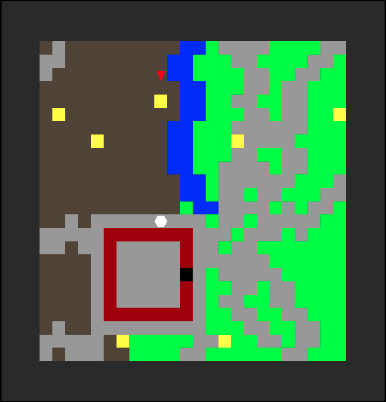
\includegraphics[scale=0.75]{belkan-1.png}
\caption{Los mundos de Belkan.}
\end{figure}
\section{Nivel 1.}

Para desarrollar el nivel 1 necesitamos utilizar un algoritmo de búsqueda para encontrar un camino al objetivo. En mi caso, utilizaré la \textbf{búsqueda por anchura}. Su pseudocódigo sería el siguiente:
\newpage


\begin{enumerate}


  \item Introducimos el origen en la cola de abiertos (por visitar)
  \item Mientras que queden elementos en abiertos o no hayamos encontrado el camino:
    \begin{enumerate}
    \item Saco el primer elemento de abiertos.
    \item Si es la solución, añado el nodo actual al histórico y salgo del bucle.
    \item En caso contrario:
      \begin{enumerate}
        \item Lo meto en cerrados (ya visitados).
        \item Para cada uno de sus adyacentes (delante,detrás,izquierda y derecha):
          \begin{itemize}      
          \item Si es viable (no está ni en abiertos ni en cerrados y es transitable), lo meto en abiertos.
          \end{itemize}
      \end{enumerate}
    \end{enumerate}
  \item Devuelvo la solución
\end{enumerate}

Consideraciones:

\begin{itemize}
  \item Como la cola de cerrados solo la utilizaremos para ver si un elemento ha sido ya explorado, la implemento mediante una matriz de booleanos. De esta forma, si quiero ver si una casilla ha sido explorada únicamente tengo que acceder al valor correspondiente de la matriz, pasando de $O(n)$ a $O(1)$ a costa de un gasto mayor de memoria. 
  \item En cuanto a la cola de abiertos, también implemento una matriz de booleanos que servirá para la operación de comprobación.
  \item Para no tener que reconstruir el camino una vez encontrada la solución, en el \textit{struct} estado he añadido una list<estado> que contenga los estados predecesores. De esta forma, una vez llegue al final solo tendré que devolver este campo (añadiendo el estado destino).
  \item Como solamente necesito conocer los antecesores de los estados que son válidos, cada vez que creo un nuevo adyacente libero la lista de antecesores de su predecesor, evitando duplicidad.
\end{itemize}

Aplicado a nuestro caso, el código sería el siguiente:

\begin{figure}[H]
\centering
\begin{minted}[linenos , breaklines]{c++}
list<estado> ComportamientoJugador::BusquedaEnAnchura
    (const estado & origen, const estado & destino) {
  queue<estado> abiertos;   // Cola de abiertos.
  abiertos.push(origen);   //Introducimos el origen
  InicializarMatrices();   // Ponemos las matrices a false.
  m_abiertos[origen.fila][origen.columna] = true;
  int dx[4] = { -1, 0, 1 , 0};  //Para calcular la adyacencia 
  int dy[4] = {0, 1, 0, -1};
  bool encontrado = false; 
  list<estado> resultado;    //Resultado a devolver

  while (!abiertos.empty() && !encontrado) {  
    estado actual = abiertos.front();  //Sacamos un estado de la cola
    abiertos.pop();
    if ( actual == destino) {  //Si hemos llegado, devolvemos 
          // los pasos que hemos seguido
      resultado = actual.anteriores;
      resultado.push_back(actual);
      encontrado = true;
    }
    else {
      m_cerrados[actual.fila][actual.columna] = true; // Añadimos a cerrados
      for (int i = 0; i < 4; i++) { //Adjustamos adyacentes
        int fila_ady = dx[i] + actual.fila;
        int col_ady = dy[i] + actual.columna;
        if (EsViable(fila_ady, col_ady)) { //Si puedo pasar por el adyacente, 
                // lo añado a la cola de abiertos
          estado adyacente = CrearAdyacente(fila_ady, col_ady, i, actual);
          abiertos.push(adyacente);
          m_abiertos[adyacente.fila][adyacente.columna] = true;
        }
      }
    }
    actual.anteriores.clear(); //Libero memoria,
    // ya que esta información estará en el adyacente.
  }
  return resultado;
}
\end{minted}
\caption{Busqueda en anchura}
\end{figure}

\begin{figure}[H]
\centering
\begin{minted}[linenos , breaklines]{c++}
bool ComportamientoJugador::EsViable(int fila, int columna) {
  return !m_abiertos[fila][columna] && !m_cerrados[fila][columna] 
  && PUEDO_PASAR.count(mapaResultado[fila][columna]);
}
\end{minted}
\caption{Es viable}
\end{figure}

PUEDO\_PASAR es un set de la \emph{STL} que contiene los valores de las casillas transitables (S,T y K).


\begin{figure}[H]
\centering
\begin{minted}[linenos , breaklines]{c++}
estado ComportamientoJugador::CrearAdyacente(int f, int c, int o, estado &actual) {
  estado adyacente;
  adyacente.fila = f;
  adyacente.columna = c;
  adyacente.orientacion = o;
  for (auto it = actual.anteriores.begin(); 
    it != actual.anteriores.end(); ++it) {
    it->anteriores.clear();   //Elimino los padres, ya que sólo necesito conservar fila, columna y orientación.
    adyacente.anteriores.push_back(*it);
  }
  adyacente.anteriores.push_back(actual);
  return adyacente;
}
\end{minted}
\caption{Crear adyacente}
\end{figure}

\begin{figure}[H]
\centering
\begin{minted}[linenos , breaklines]{c++}
void ComportamientoJugador::InicializarMatrices() {
  for (int i = 0; i < TAM; i++) {
    for (int j = 0; j < TAM; j++) {
      m_cerrados[i][j] = false;
      m_abiertos[i][j] = false;
    }
  }
}
\end{minted}
\caption{Inicializar matrices}
\end{figure}

\begin{figure}[H]
\centering
\begin{minted}[linenos , breaklines]{c++}
bool operator==(const estado &uno, const estado &otro) {
  return uno.fila == otro.fila && uno.columna == otro.columna;
}

bool operator!=(const estado &uno, const estado &otro) {
  return !(uno == otro);
}
\end{minted}
\caption{Operadores lógicos}
\end{figure}

Una vez llegados a este punto, hemos encontrado una secuencia de estados que nos llevan desde el origen hasta el destino. Por tanto, lo único que resta es transformarlos a las acciones que deberá llevar a cabo nuestro personaje. Para ello, cogeremos los elementos de la lista de dos en dos e iremos añadiendo las acciones en función de la orientación.

\begin{minted}[linenos , breaklines]{c++}
list<Action> ComportamientoJugador::calcularListaAcciones(const list<estado> &lista) {
  list<Action> resultado;
  list<estado>::const_iterator it_anterior;
  list<estado>::const_iterator it_siguiente;
  for (it_siguiente = it_anterior = lista.begin(); *it_siguiente != lista.back() ; ++it_anterior) {    //Dos iteradores: anterior y siguiente.
    ++it_siguiente;
    //Cuatro  casos: avanzo, giro izquierda , giro derecha o retrocedo
    if (it_anterior->fila > it_siguiente->fila)  {  //ARRIBA
      switch (it_anterior->orientacion) {
      case 0:     //Estoy mirando al norte
        break;
      case 1:      //Este
        resultado.push_back(actTURN_L);
        break;
      case 2:      //Sur
        resultado.push_back(actTURN_R);
        resultado.push_back(actTURN_R);
        break;
      case 3:      //Oeste
        resultado.push_back(actTURN_R);
        break;
      }
    }
    else if (it_anterior->fila < it_siguiente->fila)  {  //ABAJO
      switch (it_anterior->orientacion) {
      case 0:     //Estoy mirando al norte
        resultado.push_back(actTURN_R);
        resultado.push_back(actTURN_R);
        break;
      case 1:      //Este
        resultado.push_back(actTURN_R);
        break;
      case 2:      //Sur
        break;
      case 3:      //Oeste
        resultado.push_back(actTURN_L);
        break;
      }
    }
    else if (it_anterior->columna > it_siguiente->columna) {  //IZQUIERDA
      switch (it_anterior->orientacion) {
      case 0:     //Estoy mirando al norte
        resultado.push_back(actTURN_L);
        break;
      case 1:      //Este
        resultado.push_back(actTURN_R);
        resultado.push_back(actTURN_R);
        break;
      case 2:      //Sur
        resultado.push_back(actTURN_R);
        break;
      case 3:      //Oeste
        break;
      }
    }
    else {    //DERECHA
      switch (it_anterior->orientacion) {
      case 0:     //Estoy mirando al norte
        resultado.push_back(actTURN_R);
        break;
      case 1:      //Este
        break;
      case 2:      //Sur
        resultado.push_back(actTURN_L);
        break;
      case 3:      //Oeste
        resultado.push_back(actTURN_R);
        resultado.push_back(actTURN_R);
        break;
      }
    }
    resultado.push_back(actFORWARD);
  }
  return resultado;
}

\end{minted}
\captionof{figure}{Transcripción a acciones}
\vspace{1cm}
Por tanto, nuestro método pathfinding sería así:

\begin{minted}[linenos , breaklines]{c++}

bool ComportamientoJugador::pathFinding(const estado & origen, const estado & destino, list<Action> &plan) {
  high_resolution_clock::time_point tantes;
  high_resolution_clock::time_point tdespues;
  duration<double> tiempo;

  plan.clear();
  tantes = high_resolution_clock::now();
  list<estado> lista = BusquedaEnAnchura(origen, destino);
  tdespues = high_resolution_clock::now();
  tiempo = duration_cast<duration<double>>(tdespues - tantes);
  cout << "Tiempo empleado en el cálculo del plan: " << tiempo.count() << "s." << endl;

  tantes = high_resolution_clock::now();
  plan = calcularListaAcciones(lista);
  tdespues = high_resolution_clock::now();
  tiempo = duration_cast<duration<double>>(tdespues - tantes);
  cout << "Tiempo empleado en la transcripción a acciones: " << tiempo.count() << "s." << endl;

  VisualizaPlan(origen, plan);
  return !lista.empty();  //True si no está vacía
}

\end{minted}
\captionof{figure}{Pathfinding}

\begin{figure}[H]
\centering
\begin{subfigure}[H]{0.85\textwidth}
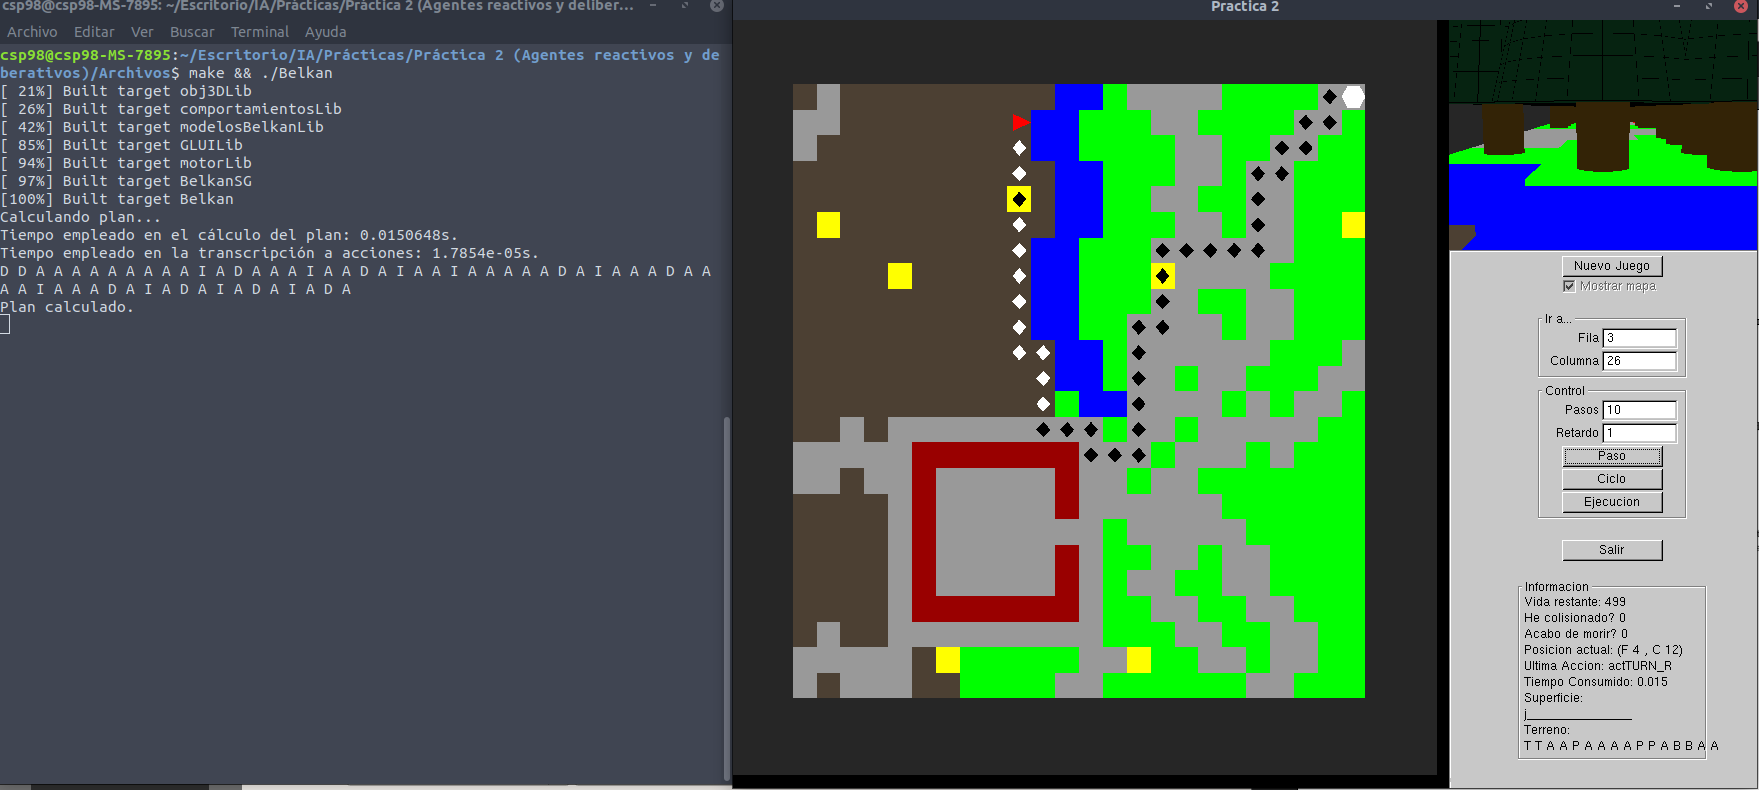
\includegraphics[width=\textwidth]{nivel_1_1.png}
\end{subfigure}
\vspace{1cm}
\begin{subfigure}[H]{0.85\textwidth}
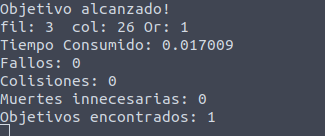
\includegraphics[width=\textwidth]{nivel_1_2.png}
\end{subfigure}
\caption{Nivel 1. Ejemplo de funcionamiento.}
\end{figure}

\newpage

\section{Nivel 2.}

En este nivel hay una serie de aldeanos que tendremos que esquivar si nos impiden el paso. La estrategia a seguir es la siguiente:

\begin{enumerate}
  \item Trazar un plan al igual que en el nivel 1.
  \item Si en el trascurso del plan encuentro un aldeano en mi camino:
    \begin{enumerate}
      \item Coloco temporalmente un muro en la posición del aldeano.
      \item Llamo de nuevo a pathfinding, generando un nuevo camino. Al haber situado un muro en la posición del aldeano, nuestro algoritmo anterior lo esquivará.
      \item Devuelvo la casilla del aldeano a su estado original.
    \end{enumerate}
\end{enumerate}

Por tanto, nuestro método \emph{think()} quedaría así:

\begin{minted}[linenos , breaklines]{c++}
Action ComportamientoJugador::think(Sensores sensores) {
  if (sensores.mensajeF != -1 && primeraVez) {
    primeraVez = false;
    fil = sensores.mensajeF;
    col = sensores.mensajeC;
  }

  // Actualizar el efecto de la ultima accion
  switch (ultimaAccion) {
  case actTURN_R: brujula = (brujula + 1) % 4; break;
  case actTURN_L: brujula = (brujula + 3) % 4; break;
  case actFORWARD:
    switch (brujula) {
    case 0: fil--; break;
    case 1: col++; break;
    case 2: fil++; break;
    case 3: col--; break;
    }
    cout << "fil: " << fil << "  col: " << col << " Or: " << brujula << endl;
    break;
  }

  // Determinar si ha cambiado el destino desde la ultima planificacion
  if (hayPlan and (sensores.destinoF != destino.fila or sensores.destinoC != destino.columna)) {
    cout << "El destino ha cambiado\n";
    hayPlan = false;
  }

  // Determinar si tengo que construir un plan
  if (!hayPlan) {
    //Capto origen y destino.
    estado origen;
    origen.fila = fil;
    origen.columna = col;
    origen.orientacion = brujula;
    destino.fila = sensores.destinoF;
    destino.columna = sensores.destinoC;

    cout << "Calculando plan..." << endl;
    hayPlan = pathFinding(origen, destino, plan);
    PintaPlan(plan);
    cout << "Plan calculado." << endl;
    if (!hayPlan)
      cout << "El objetivo es inalcanzable." << endl;
  }


  // Ejecutar el plan
  Action sigAccion;
  if (hayPlan and plan.size() > 0) {
    sigAccion = plan.front();
    plan.erase(plan.begin());

    if (sigAccion == actFORWARD and sensores.superficie[2] == 'a') {
      int f_aux = fil;
      int c_aux = col;

      estado origen;
      origen.fila = fil;
      origen.columna = col;
      origen.orientacion = brujula;

      destino.fila = sensores.destinoF;
      destino.columna = sensores.destinoC;

      //Calculo la posición del aldeano.
      switch (brujula) {
      case 0:
        f_aux--;
        break;
      case 1:
        c_aux++;
        break;
      case 2:
        f_aux++;
        break;
      case 3:
        c_aux--;
        break;
      }
      // Arreglo temporal: pongo un muro en el lugar del aldeano para que no sea transitable y no tener que modificar pathFinding()
      char aux = mapaResultado[f_aux][c_aux];
      mapaResultado[f_aux][c_aux] = 'M';

      cout << "Recalculando ruta..." << endl;

      hayPlan = pathFinding(origen, destino, plan);
      
      mapaResultado[f_aux][c_aux] = aux;

      PintaPlan(plan);
      cout << "Plan calculado." << endl;

      if (!plan.empty()) {      //Si el plan no está vacío, saco la primera acción. En caso contrario, espero.
        sigAccion = plan.front();
        plan.erase(plan.begin());
      }
      else {
        sigAccion = actIDLE;
      }
    }
  }
  else {
    sigAccion = actIDLE;
  }
  ultimaAccion = sigAccion;
  return sigAccion;
}

\end{minted}
\captionof{figure}{Think}

\begin{figure}[H]
\centering
\begin{subfigure}[H]{0.85\textwidth}
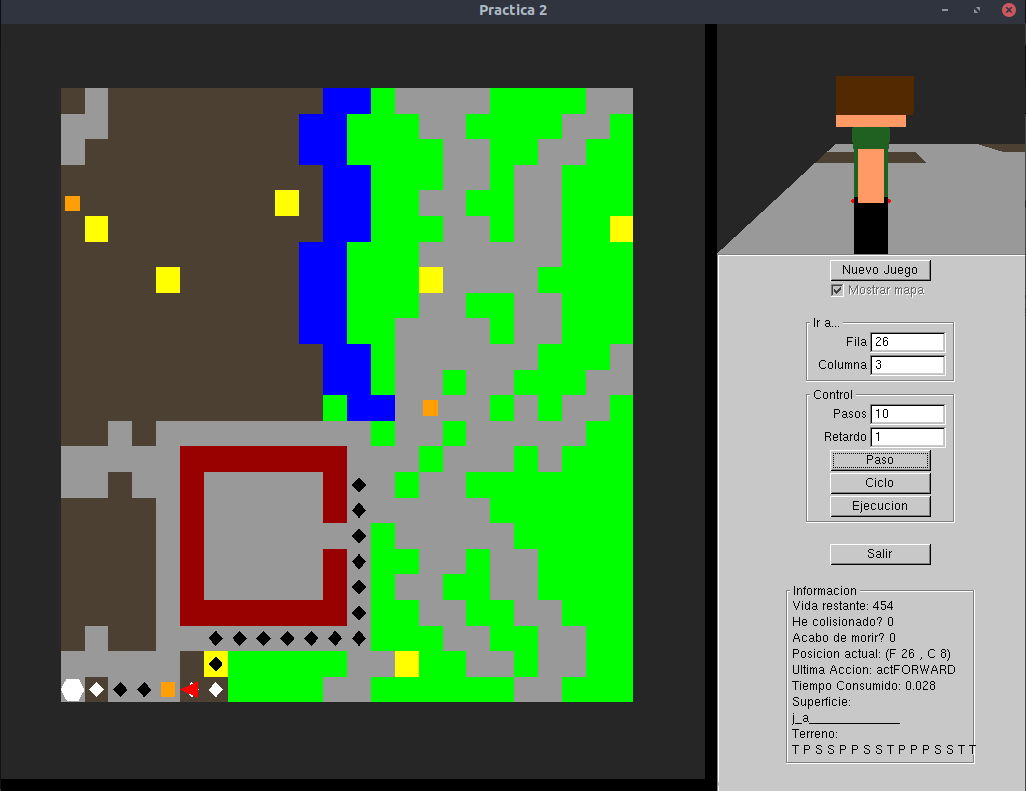
\includegraphics[width=\textwidth]{nivel_2_1.png}
\end{subfigure}
\vspace{1cm}
\begin{subfigure}[H]{0.85\textwidth}
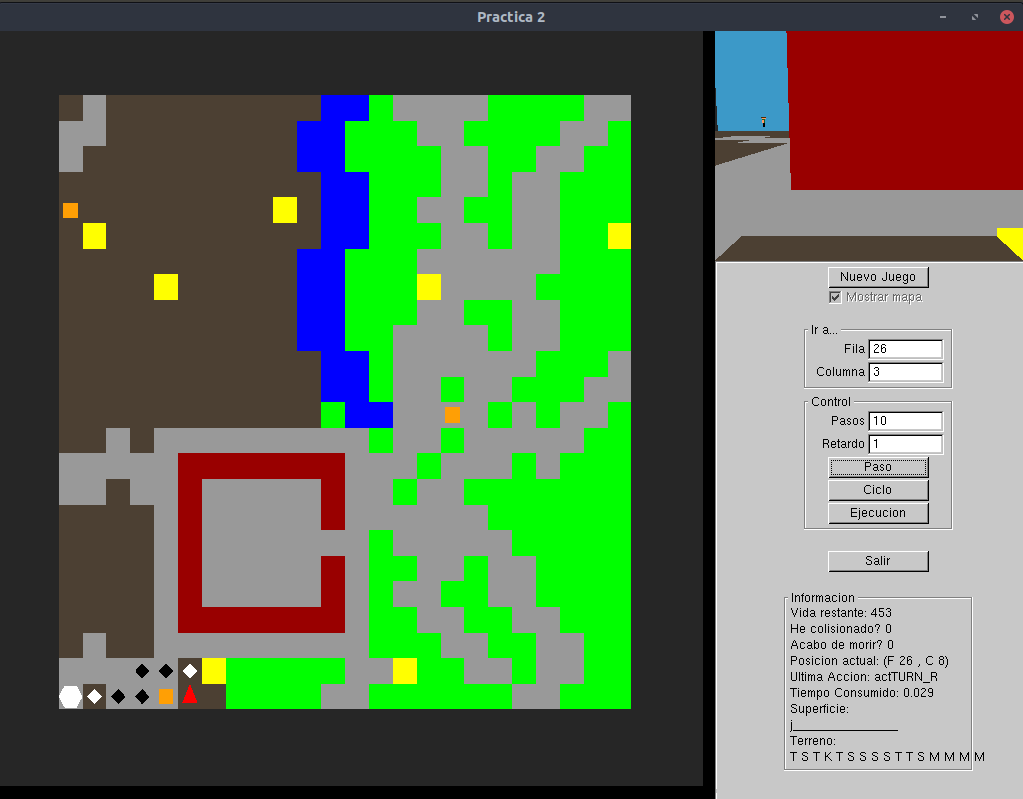
\includegraphics[width=\textwidth]{nivel_2_2.png}
\end{subfigure}
\caption{Nivel 2. Ejemplo de funcionamiento.}
\end{figure}


\end{document}
